\section{Klassen und Objekte}

\noindent
\textbf{Klassen} sind Abstraktionen von Objekten.\\

\noindent
\textbf{Objekte} besitzen Eigenschaften und Verhalten.\\

\noindent
In der \textbf{UML} werden Attribute und Verantwortlichkeiten oder Operationen in \textbf{Compartments} (dt. \textit{Abteilungen}) dargestellt.\\

\noindent
Einschränken des Typs können hinter dem Typ in der \textbf{Object Constraint Language}\footnote{
s. Version 2.4: \url{https://www.omg.org/spec/OCL}, abgerufen 11.04.2024
} (\textbf{OCL}) angegeben werden.\\
Diese Angaben - oder als Kommentar in Textform angegeben - ersetzen im \textit{Klassendiagramm der Analyse} das \textbf{Datadictionary} (s. Abschnitt~\ref{sec:datadictionary-und-mengengerust}) (s. Abbildung~\ref{fig:moneyocl}).

\begin{figure}
    \centering
    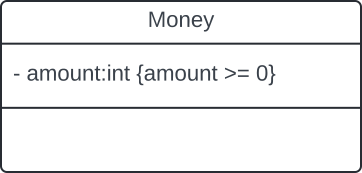
\includegraphics[scale=0.4]{part two/Objektorientierte Analyse/img/moneyocl}
    \caption{Die OCL-Notation in Verbindung mit einem UML-Klassendiagramm zur Spezifizierung des Wertebereichs des Attributes \textit{amount}. (Quelle: eigene)}
    \label{fig:moneyocl}
\end{figure}